\section{Problems and core issues of the current system} \label{sec:as-is-issues}
The analysis of the architecture and workflow of the current SRP system has revealed a number of critical issues that compromise its scalability, maintainability, and reliability. These problems are deeply rooted in the technological and design choices made years ago and are evident across several key areas of the system, from catalog management to script execution and the import of master data from Active Directory.

\subsection{Architectural and Technological Challenges}

The SRP system is characterized by a fragmented architectural structure and complex interdependencies between its main components, which leads to several critical issues.

\subsubsection{Monolithic Frontend Component}
The user interface, responsible for navigating the Service Request catalog and completing the associated forms, is an excessively large and complex Vue.js frontend component (nearly 11,000 lines). This architecture makes modifications, extensions, and client-specific customizations exceptionally challenging \cite{benefits_issues_micro_frontends}. The logic for managing dynamic fields, their interdependencies, and the rules for compilation and validation are all handled at the frontend level through a long series of hard-coded conditional statements, such as the following:

\begin{minted}[linenos,tabsize=2,breaklines]{vue}
<div v-if="field.desc == 'Domain'">
    ...
</div>
\end{minted}

This, in addition to mixing business logic with presentation, represents a significant challenge for catalog configuration, as there is no centralized way to manage the fields and their relationships. Every change, therefore, requires a direct intervention on the code, making the system inflexible and difficult to maintain, especially in a context where the operator modifying the catalog is not a programmer and does not know how the frontend code is structured. For instance, if an operator wanted to add a new "Domain" field to a Service Request, this field would need to have the exact description "Domain" and type "domain"; otherwise, the Vue.js component would not render it correctly.

These dynamics make the system fragile and susceptible to frequent errors that waste time and resources for both clients and operators \cite{benefits_issues_micro_frontends}.

\subsubsection{Overly Generic Backend REST Service}

The only information about the fields returned by the backend REST service (\texttt{SRPWebSeviceREST}), besides the field name and its mandatoriness, is its \textit{type}. It is therefore easy to imagine how this information, which should only be an indication of the component that needs to be rendered (e.g., textbox, select, radio button, etc.), can become an identifier for something much broader.

For example, a field of type \texttt{UPN} is a composite field derived from the value of another field, '\texttt{Display Name}', concatenated with an '\texttt{@}' symbol, and suffixed with the value from a select field whose options are the client's domains, provided by an external REST service (e.g., "\texttt{n.guarini@elmec.it}", where "\texttt{n.guarini}" is the value of the "\texttt{Display Name}" field, and "\texttt{elmec.it}" is the value of the "\texttt{Domain}" select field). 

Despite this complexity, the REST service returns only a JSON document of this type:

\begin{minted}[linenos,tabsize=2,breaklines]{json}
{
    "idField": 1603,
    "descField": "UPN",
    "type": "upn",
    "mandatory": true
}
\end{minted}

thus delegating to the frontend the responsibility of interpreting the type and rendering the field correctly.

\subsubsection{Dependency on the SRP Agent}

The import of data from clients' Active Directories and the actual execution of Service Requests are handled by an agent (\texttt{SRPWindowsService}) installed directly on the clients' Domain Controllers. This approach presents several challenges:

\begin{itemize}
    \item \textbf{Security and Permissions}: The agent often requires credentials with elevated privileges (e.g., \texttt{domain-admin}), which clients are increasingly reluctant to grant.
    \item \textbf{Reliability and Control}: The configurations on the agent and the Domain Controller are complex and difficult to manage centrally, which can cause execution errors and data synchronization issues.
    \item \textbf{Scalability}: The need to install, configure, and maintain an agent for each client domain represents a significant operational effort. Alternatives such as more modern provisioning systems will be evaluated.
    \item \textbf{Obsolete Communication Patterns}: The unidirectional communication through the \textit{DMI Console} creates a bottleneck and complicates the management of asynchronous operations. Communication between components in the client's network and the company network is based on polling (e.g., the SRP Agent queries the server every 5 minutes), an approach that introduces latency and inefficiencies.
\end{itemize}

\subsection{Code and Data Management Issues}

Code and data persistence management is another critical aspect of the system, characterized by a lack of versioning and modern debugging tools.

\subsubsection{Unversioned and Undebuggable Stored Procedures}
The intensive use of Stored Procedures\footnote{Stored procedures are SQL code routines, or sets of instructions, that are pre-compiled and stored within a relational database. They act as logical units of execution, encapsulating business logic directly at the database level \cite{stored-procedures}.} in the MSSQL database represents one of the major weaknesses. These procedures contain fundamental business logic and are:
\begin{itemize}
    \item \textbf{Unversioned}: There is no centralized version control system for Stored Procedures. Changes are made directly on the database, making it impossible to track changes, revert to previous versions, or test modifications in separate environments.
    \item \textbf{Difficult to Debug}: Debugging Stored Procedures is a complex and cumbersome process, often requiring direct access and specific SQL server tools, with the risk of affecting the production environment.
\end{itemize}

\subsubsection{Inaccessible and Unversioned SSIS Jobs}
SSIS packages\footnote{SQL Server Integration Services (SSIS) is a platform for building data integration and workflow solutions. It is a key component of Microsoft SQL Server, primarily used for Extract, Transform, Load (ETL) operations, enabling the extraction of data from various sources, its transformation, and its loading into different destinations \cite{ssis}.} are essential for data import and export operations (e.g., AD master data). However, these jobs reside physically on the \texttt{ELMEC-CMI-MSSQL} server, and the only way to access and modify them is via a remote desktop. This approach prevents versioning and collaboration, limits accessibility by making maintenance and debugging an onerous and risky activity, and creates a \textit{single-point-of-failure} and a strong coupling between the import/export business logic and the infrastructure.

\subsection{Database Schema and Data Integrity Issues}

\begin{figure}[htbp]
    \centering
    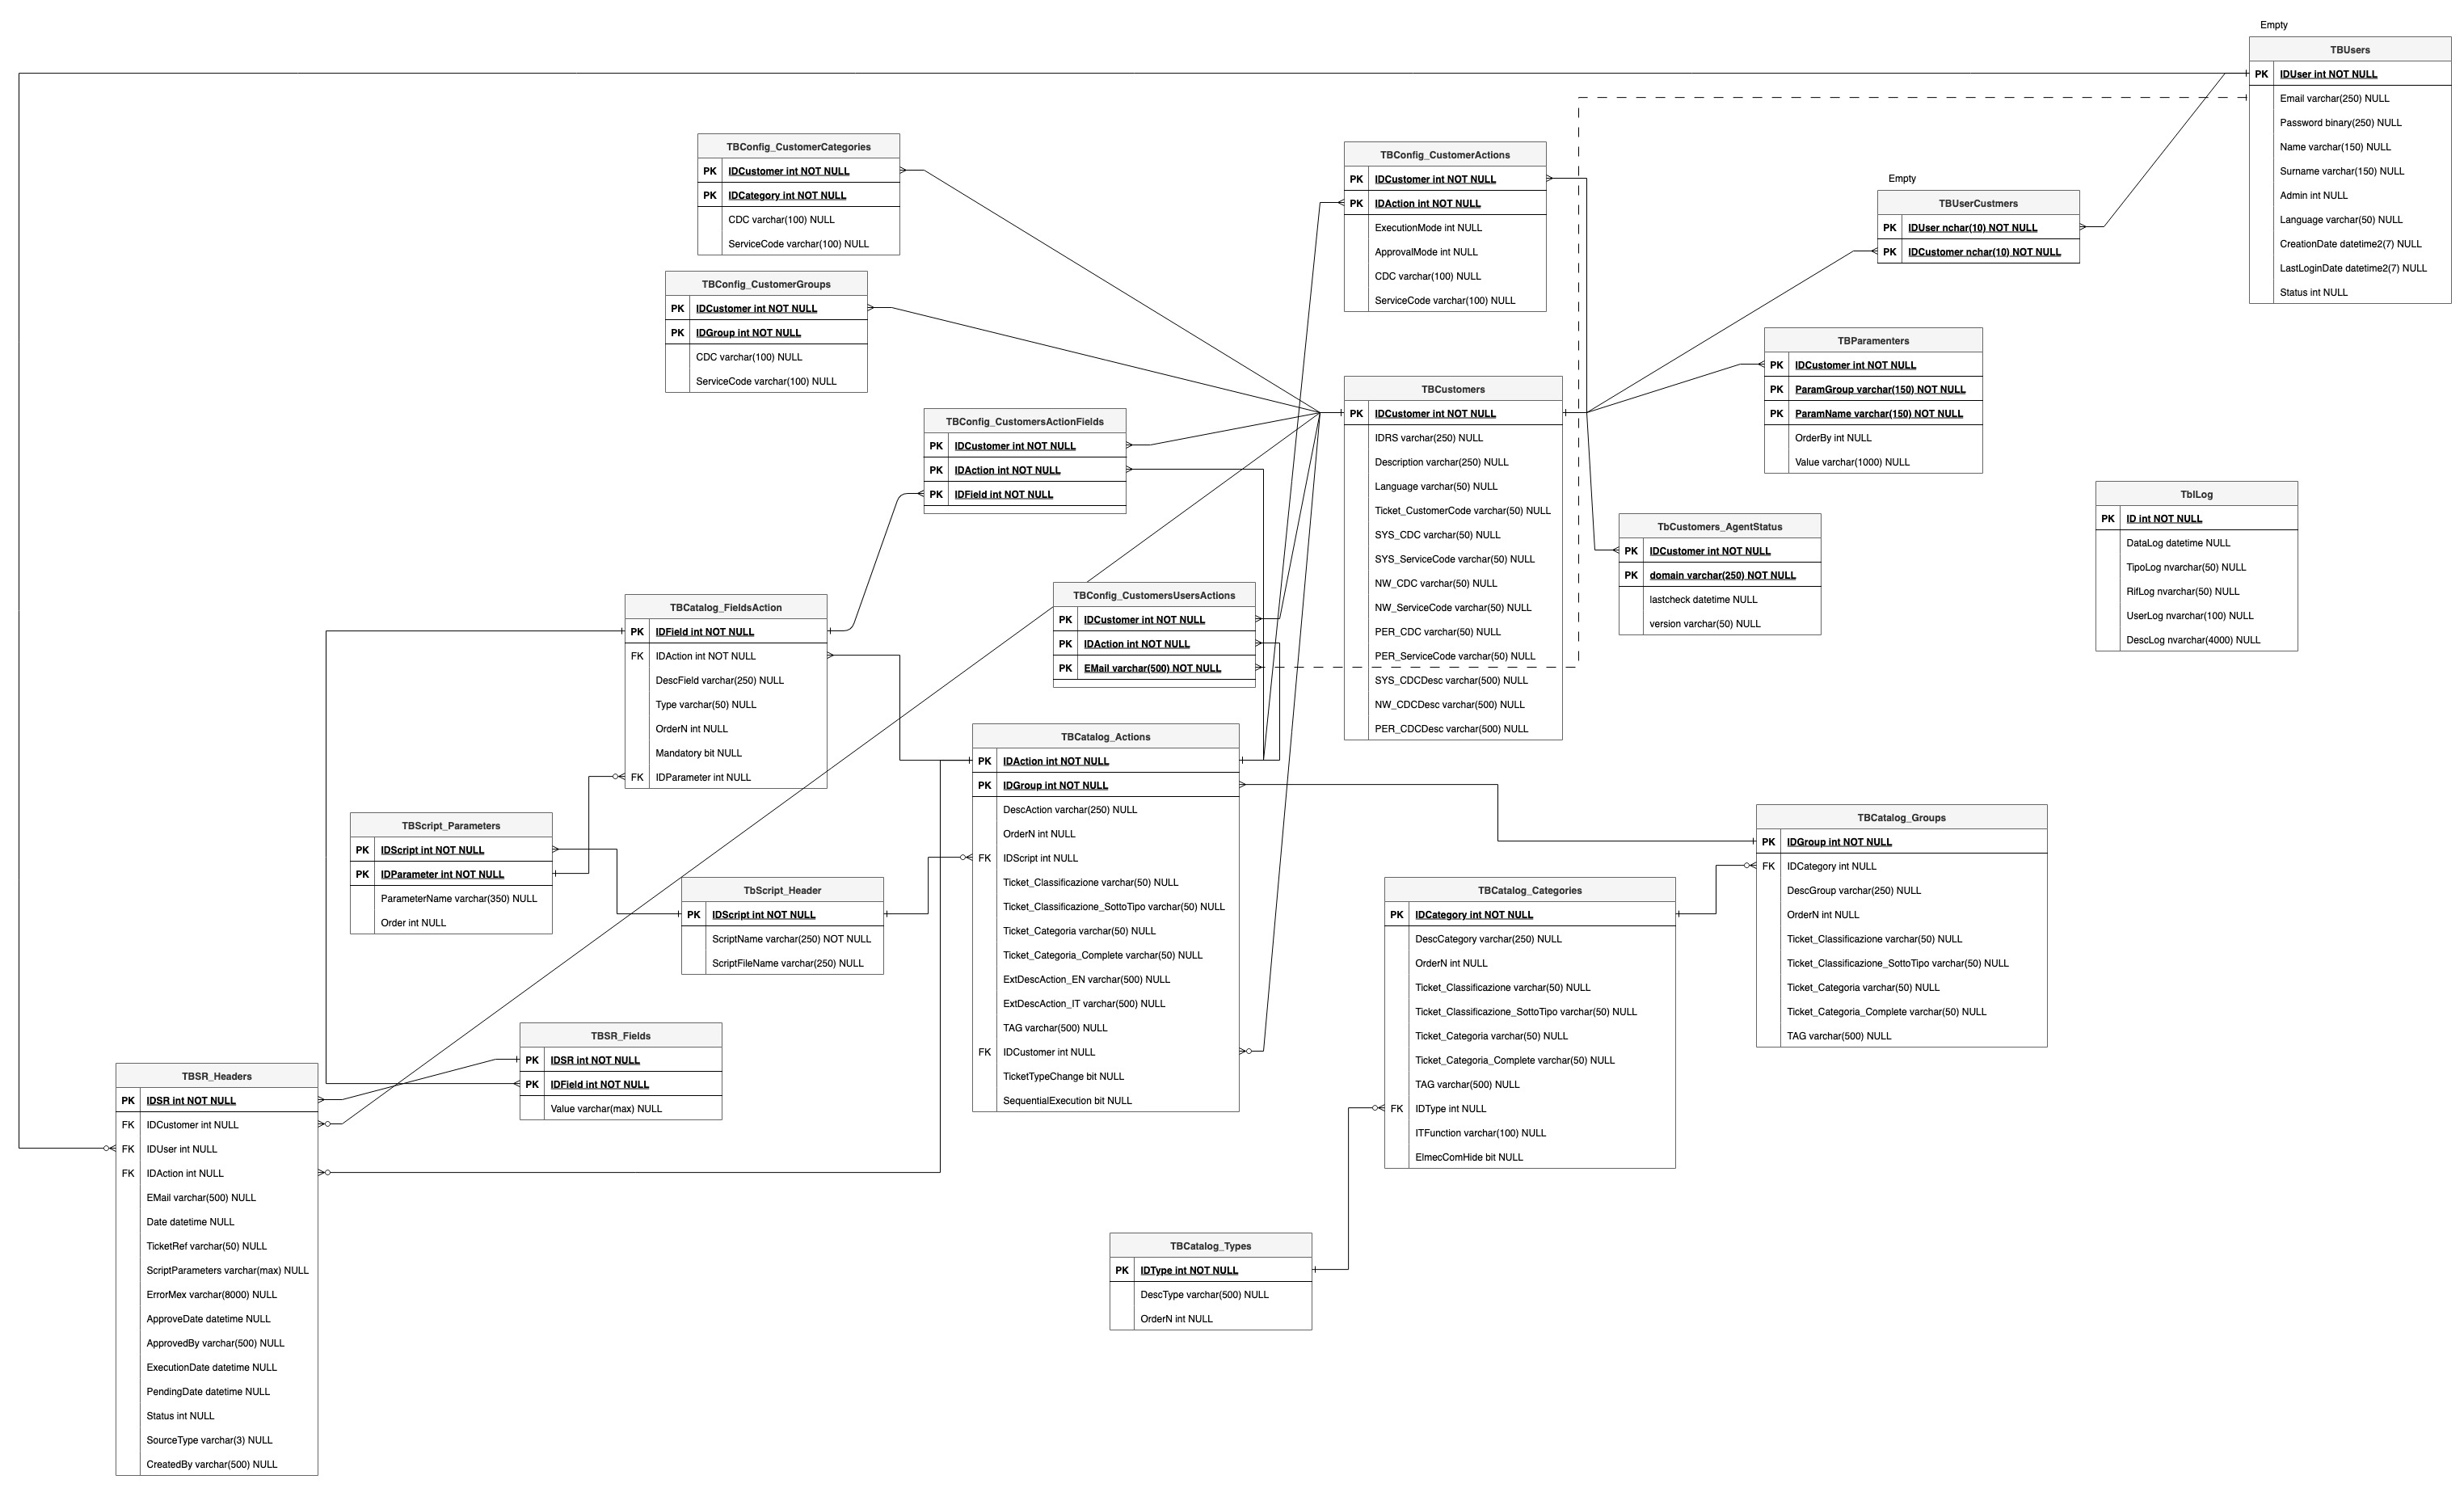
\includegraphics[width=\textwidth, keepaspectratio]{images/as-is/ER SRM-SRP AS-IS.jpg}
    \caption{AS-IS Database ER Schema}
    \label{fig:er-as-is}
\end{figure}

%\begin{figure}[htbp]
%    \centering
%    \includegraphics[width=\textwidth, keepaspectratio]{images/as-is/%srp_er_customers.png}
%    \caption{AS-IS Database ER Schema (Admin / Customers)}
%    \label{fig:er-as-is-customers}
%\end{figure}
%
%\begin{figure}[htbp]
%    \centering
%    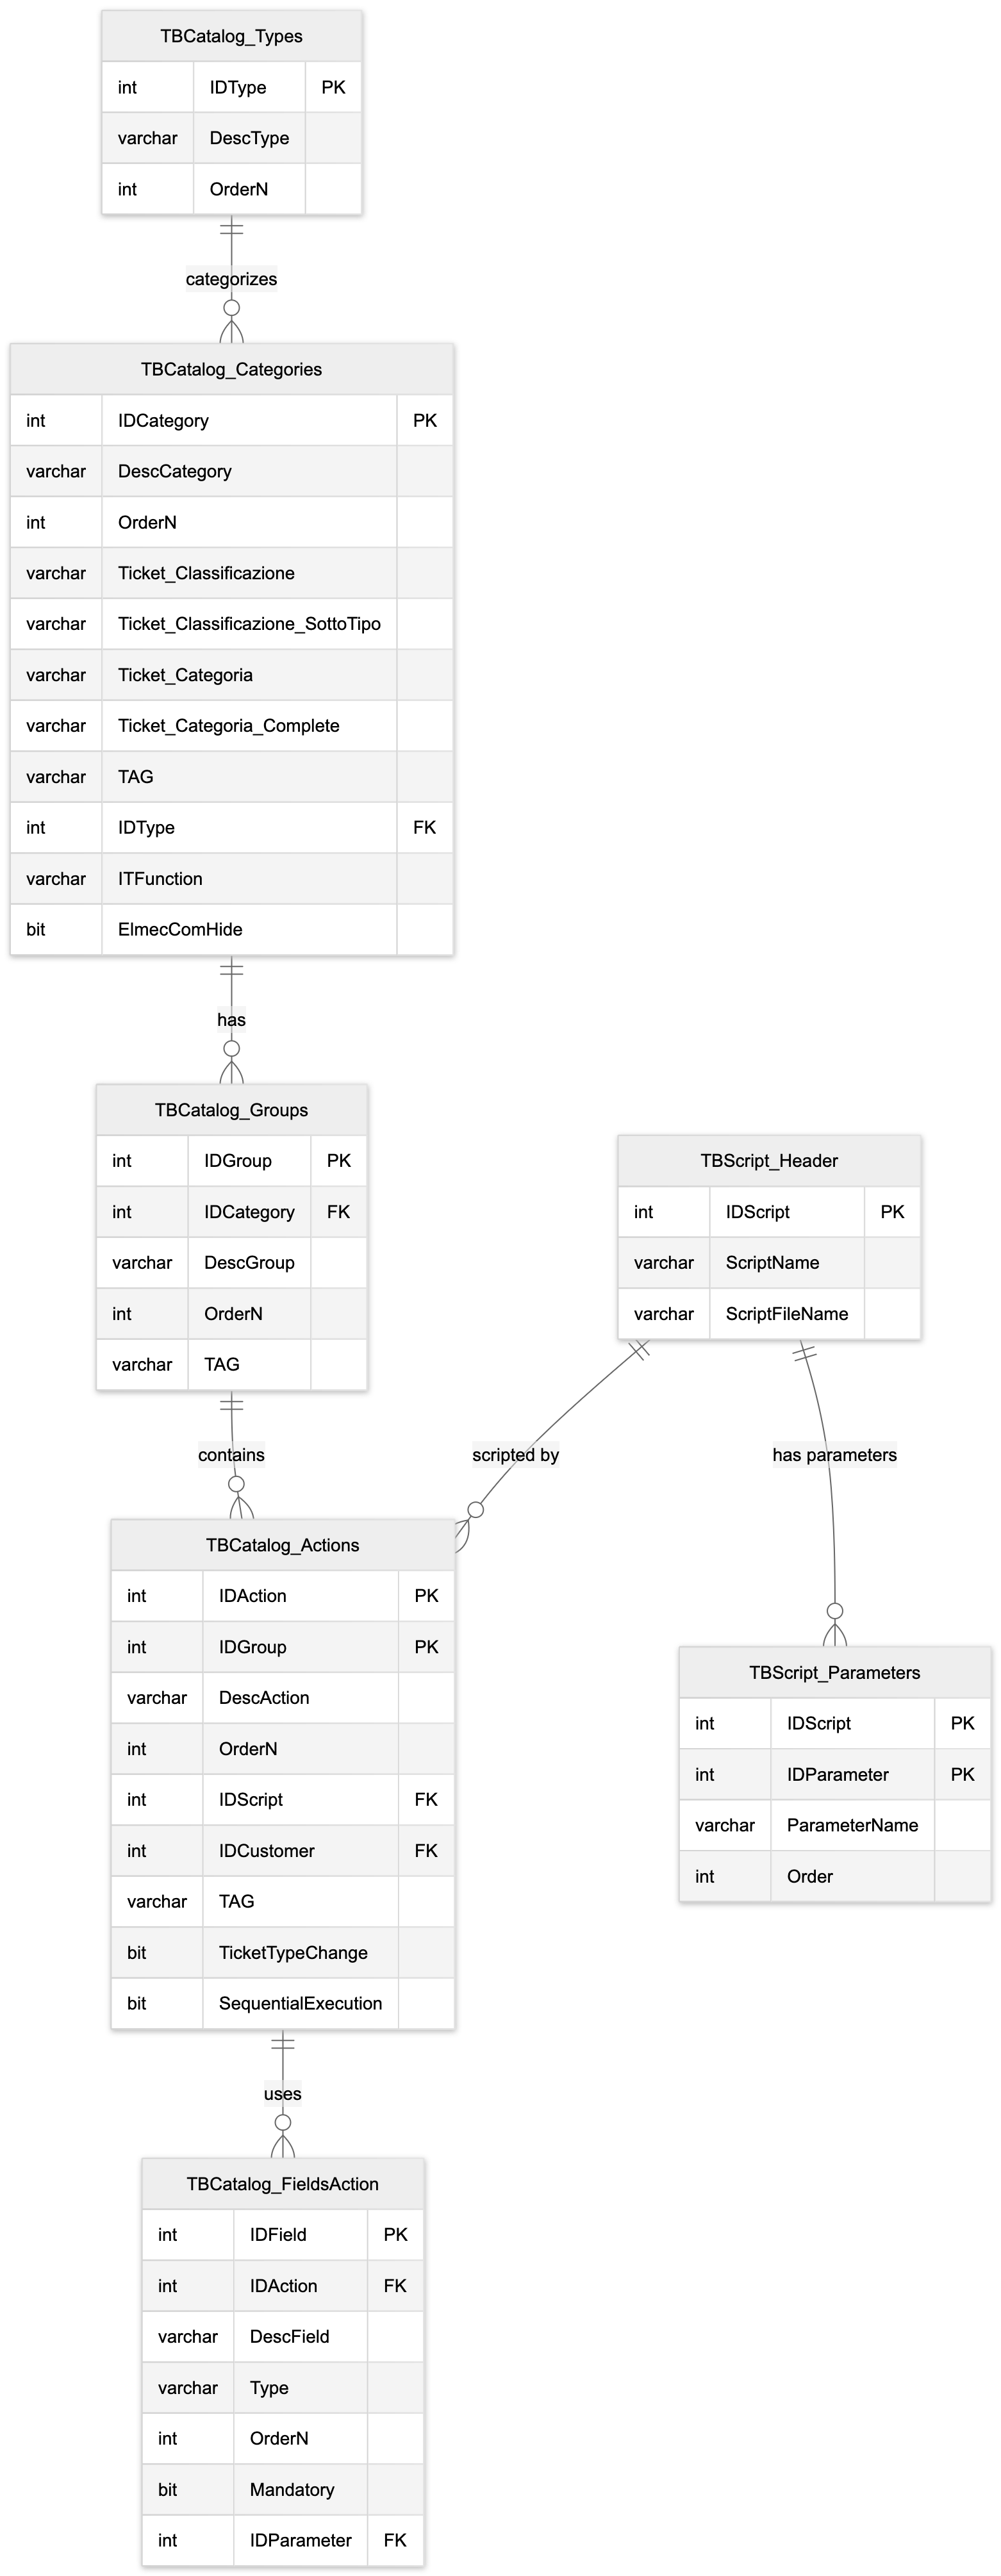
\includegraphics[width=0.6\textwidth]{images/as-is/srp_er_actions.png}
%    \caption{AS-IS Database ER Schema (Catalog / Actions)}
%    \label{fig:er-as-is-actions}
%\end{figure}
%
%\begin{figure}[htbp]
%    \centering
%    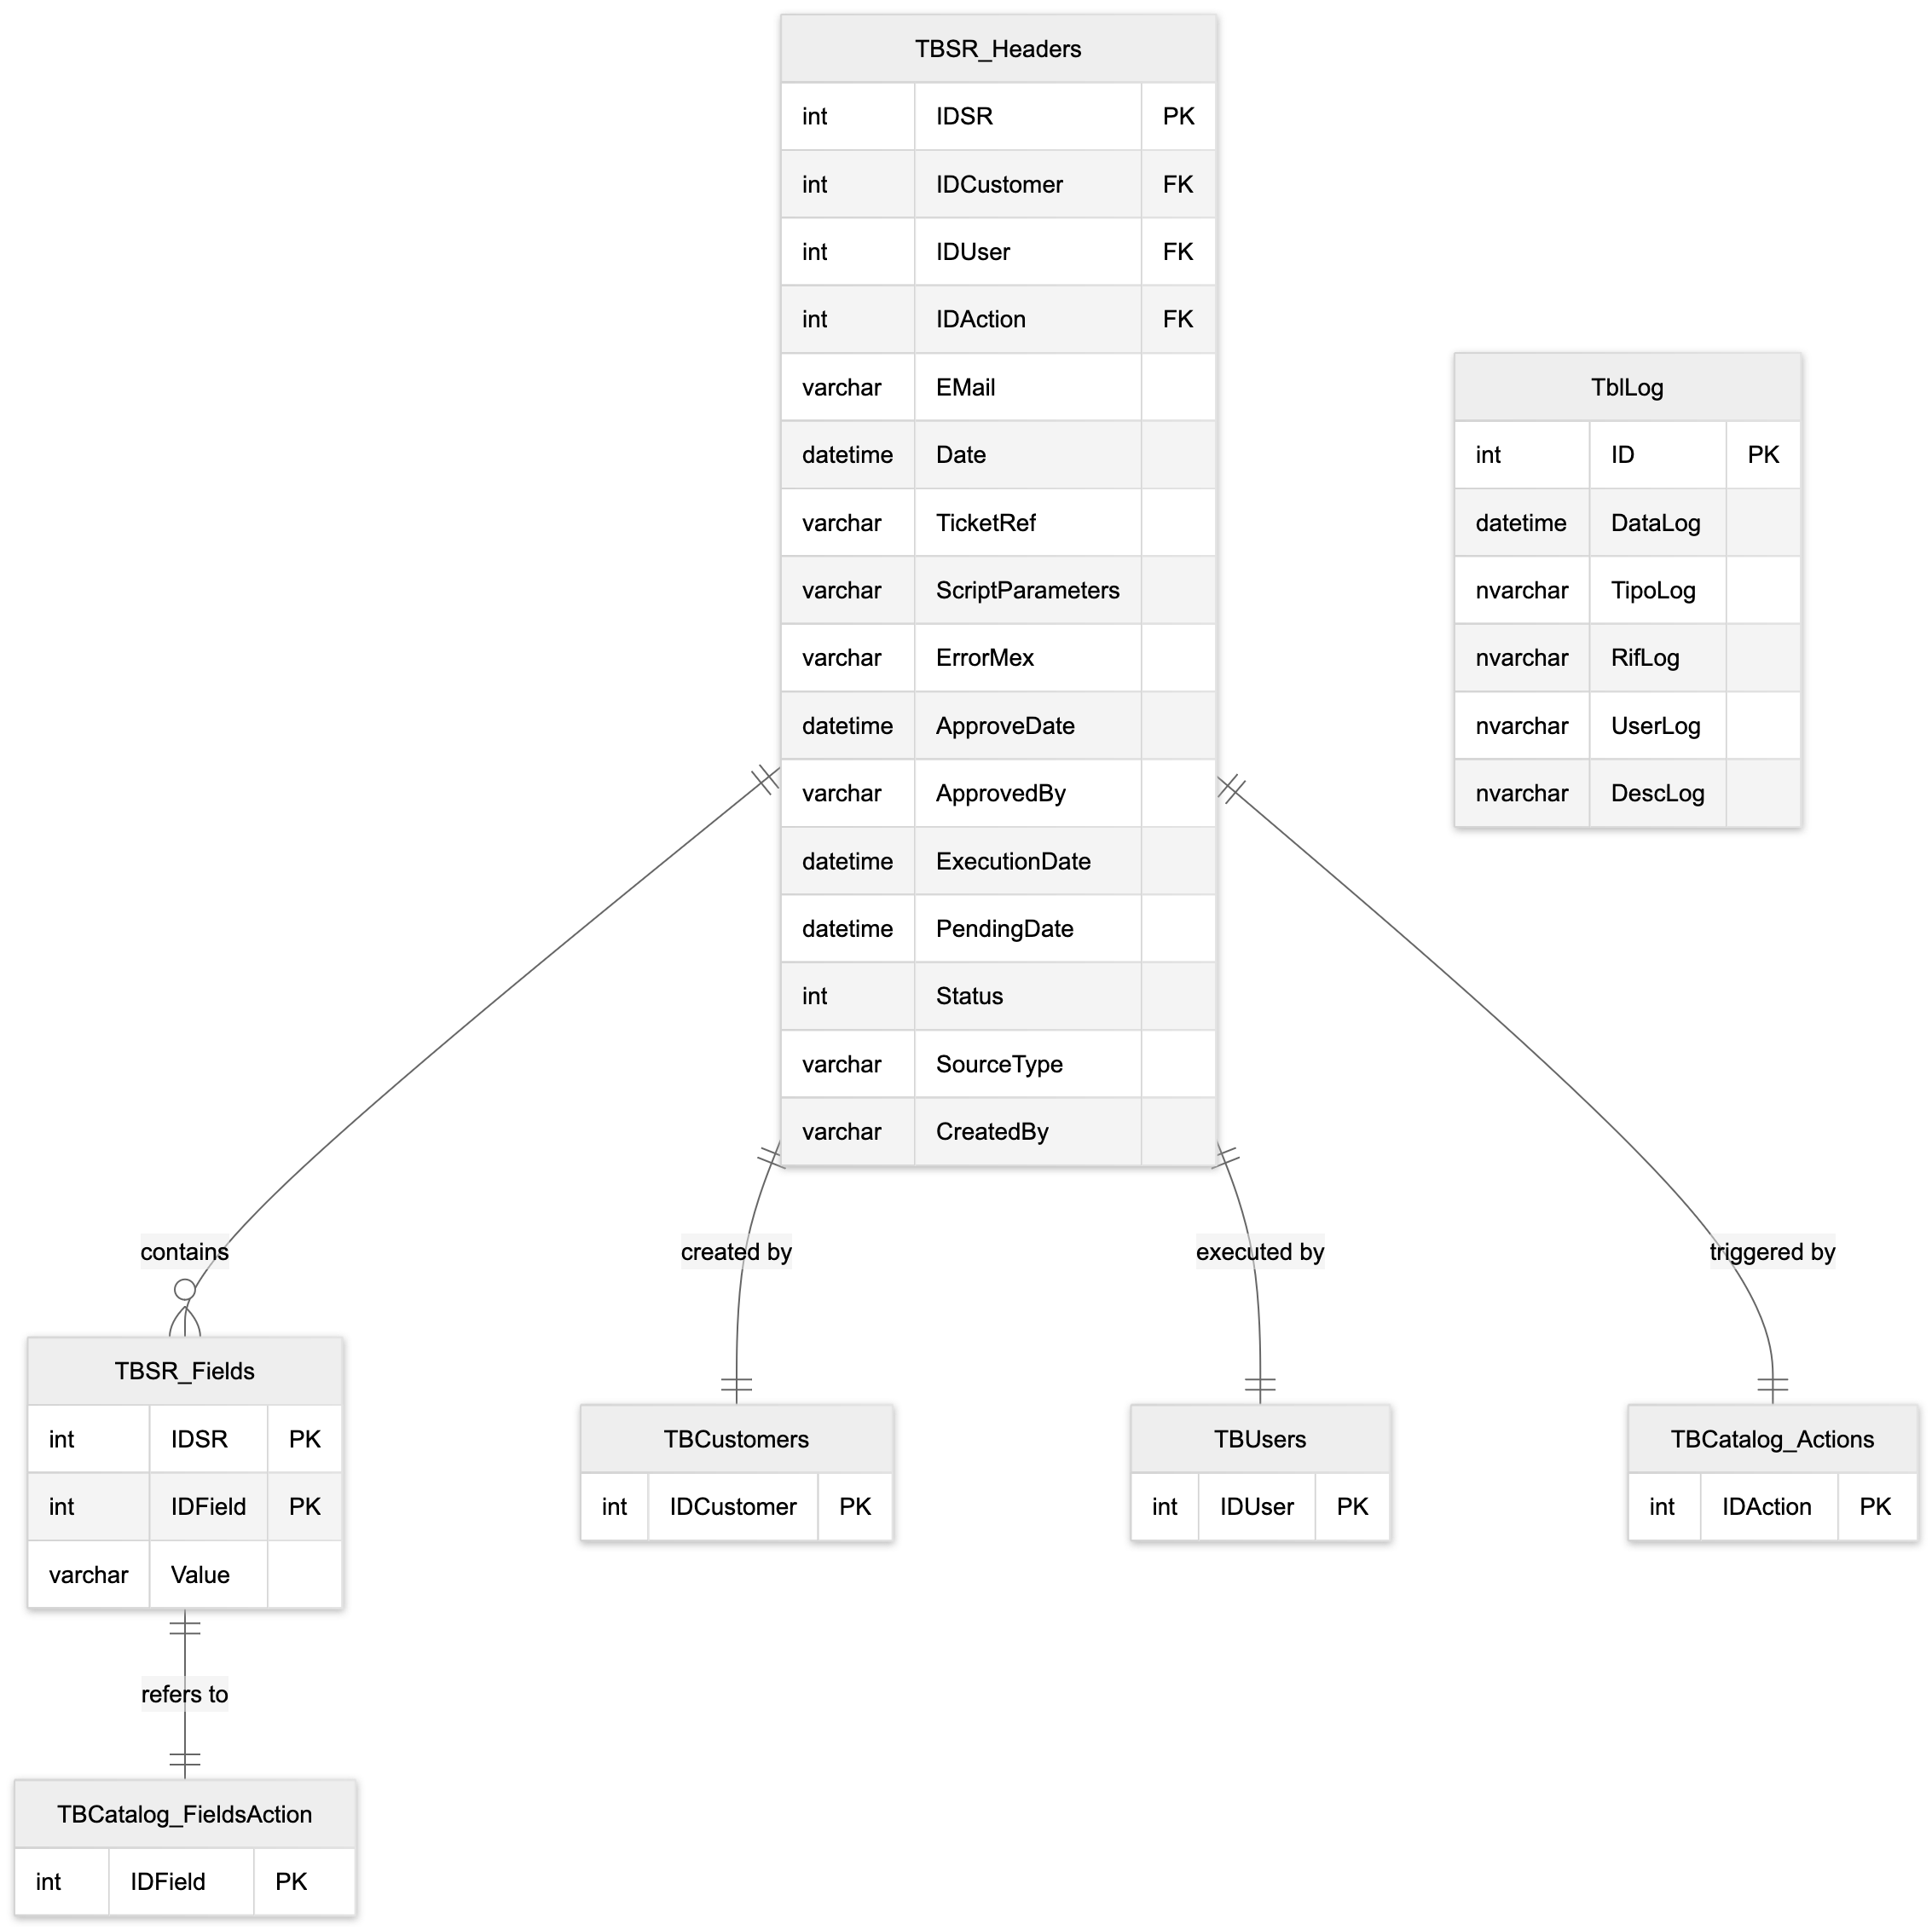
\includegraphics[width=1\textwidth]{images/as-is/srp_er_execution.png}
%    \caption{AS-IS Database ER Schema (Execution / Service Requests)}
%    \label{fig:er-as-is-execution}
%\end{figure}

The analysis of the database schema, represented in figures \ref{fig:er-as-is}, has revealed a number of significant issues that affect the quality and integrity of the data managed by the SRP system.

\subsubsection{Lack of Data Integrity and Consistency}
One of the most significant problems concerns the lack of explicit referential integrity constraints. In the schema in figure \ref{fig:er-as-is}, although the relationships between tables have been inferred manually, they are not defined at the database level through the use of foreign keys. This absence prevents the database from guaranteeing data integrity \cite{referential_integrity_important_databases}: for example, a row in a child table could refer to a non-existent row in the parent table \cite{referential_integrity_y42}. Such a scenario, known as a "dangling reference\footnote{The "dangling pointer" is a problem typically addressed in the context of low-level programming, where a pointer refers to a memory area that is no longer valid because it has been freed or because the pointer is used outside the context of the variable's existence to which it refers \cite{apogeo-fondamenti-programmazione}, but the same dynamic can also be applied in the context of databases, where the "pointers" are represented by foreign keys.}", can generate anomalies and inconsistencies in the system, making the data unreliable and debugging extremely complex \cite{referential_integrity_important_databases}.

\subsubsection{Data Redundancy}
Another issue is the high data redundancy and the large number of duplicate attributes across different tables \cite{srp_windowsservice_git}. This design, which deviates from the principles of normalization \cite{technical_debt_is_database_normalization}, leads to storing the same information in multiple locations, which not only increases the data volume but also introduces a high risk of inconsistencies \cite{technical_debt_is_database_normalization}.

\subsubsection{Unclear and Inconsistent Naming Conventions}
The naming convention for attributes and tables is inconsistent and unclear. The schema presents a mixture of conventions (e.g., \texttt{IDGroup} vs. \texttt{GroupID}, English names mixed with specific terms) and typos (e.g., \texttt{TBParamenters}), making it difficult to immediately understand the function of each field. In many cases, the naming is not explicit enough to describe the role of an attribute, requiring an in-depth knowledge of the system to correctly interpret the relationships and business logic. This lack of a unique and standardized vocabulary hinders collaboration among developers, complicates code maintenance, and increases the likelihood of errors.

\subsection{Maintenance and Operational Challenges}

According to information discussed in an internal meeting \cite{requirements_meeting}, the daily management of the system is made complex by several inefficiencies and obsolete design choices.

The current system design does not allow for the effective reuse of Service Requests and catalog configurations. Consequently, every modification or addition requires the creation of a new Service Request, even for small variations, leading to a innefficient and difficult-to-manage catalog, consisting of numerous duplicate SRs and fields. This, while functional, is not a scalable approach and leads to significant inefficiencies in catalog management itself. For example, if a Service Request needs to be modified for all clients who use it, the operator will have to modify not only the SR in question but also all the duplicate SRs for each client, with the risk of forgetting a modification or making mistakes. This approach, although probably conceived to prevent error propagation, makes the catalog difficult to navigate and maintain.

The new architecture will need to address these challenges by introducing a more robust, versioned system based on modern software design principles and patterns.